%%%% cs420.tex

\typeout{CS420 Course Project Report Template}

% This file is the template for CS420 course project report.
% It is based on the instructions for authors for IJCAI-19.

\documentclass{article}
\pdfpagewidth=8.5in
\pdfpageheight=11in
\usepackage{cs420}

% Use the postscript times font!
\usepackage{times}
\usepackage[hidelinks]{hyperref}
\usepackage[utf8]{inputenc}
\usepackage[small]{caption}
\usepackage{graphicx}
\usepackage{amsmath}
\usepackage{booktabs}
\usepackage{float}
\urlstyle{same}

% the following package is optional:
%\usepackage{latexsym} 

% Following comment is from ijcai97-submit.tex:
% The preparation of these files was supported by Schlumberger Palo Alto
% Research, AT\&T Bell Laboratories, and Morgan Kaufmann Publishers.
% Shirley Jowell, of Morgan Kaufmann Publishers, and Peter F.
% Patel-Schneider, of AT\&T Bell Laboratories collaborated on their
% preparation.

% These instructions can be modified and used in other conferences as long
% as credit to the authors and supporting agencies is retained, this notice
% is not changed, and further modification or reuse is not restricted.
% Neither Shirley Jowell nor Peter F. Patel-Schneider can be listed as
% contacts for providing assistance without their prior permission.

% To use for other conferences, change references to files and the
% conference appropriate and use other authors, contacts, publishers, and
% organizations.
% Also change the deadline and address for returning papers and the length and
% page charge instructions.
% Put where the files are available in the appropriate places.

\title{Text-Classification Report }

% Single author syntax
\author{
    Yuxuan Chen
    \affiliations
    Zhiyuan College, Shanghai Jiao Tong University \emails
    chenyxuan@sjtu.edu.cn
}

% Multiple author syntax (remove the single-author syntax above and the \iffalse ... \fi here)
% Check the ijcai19-multiauthor.tex file for detailed instructions
\iffalse
\author{
First Author$^1$
\and
Second Author$^2$\and
Third Author$^{2,3}$\And
Fourth Author$^4$
\affiliations
$^1$First Affiliation\\
$^2$Second Affiliation\\
$^3$Third Affiliation\\
$^4$Fourth Affiliation
\emails
\{first, second\}@example.com,
third@other.example.com,
fourth@example.com
}
\fi

\begin{document}

\maketitle

\begin{abstract}
This paper provides the report of text-classification project of CS420 Machine Learning, including models selection, model design and experiments. 
\end{abstract}

\section{Introduction}
\quad This project is mainly a text classification task, which aims to predict the probability of the given review text to be positive (binary classification). Our goal is to train a classification model that provide estimated probability given the review text.

\section{Non-Sequential Models}
\quad As a tentative idea, we focus on the frequency of each word and apply TF-IDF to raw corpus. Now we can regard each instance 
\textsl{(senence, label)} as \textsl{(point, label)}. Now the problem comes to do binary classification in hyperspace.

\subsection{K-Nearest Neighbor}
\quad K nearest neighbors is a simple algorithm that stores all available cases and classifies new cases based on a similarity measure (e.g., distance functions). KNN has been used in statistical estimation and pattern recognition already in the beginning of 1970’s as a non-parametric technique.

After several experiments, K = 27 shows the best performance. ROC of KNN is blue.

\begin{figure}[H]
\centering
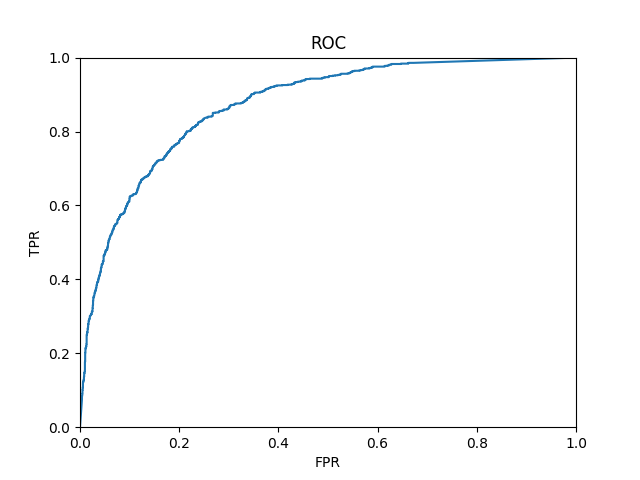
\includegraphics[width=.4\textwidth]{KNN.png}
\caption{K-Nearest Neighbor}
\end{figure}

\subsection{Multilayer Perceptron Classifier}
\quad Multilayer perceptron classifier (MLPC) is a classifier based on the feedforward artificial neural network. MLPC consists of multiple layers of nodes. Each layer is fully connected to the next layer in the network. Nodes in the input layer represent the input data. All other nodes map inputs to outputs by a linear combination of the inputs with the node’s weights w and bias b and applying an activation function. 

As is shown below, there is a sharp contrast between MLPC and KNN. ROC of MLPC is orange.

\begin{figure}[H]
\centering
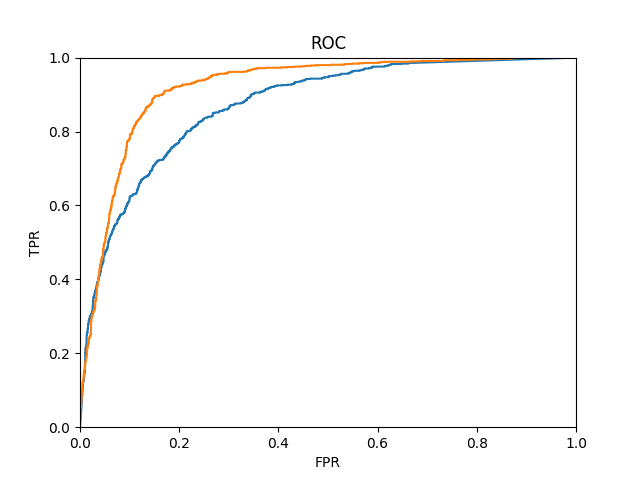
\includegraphics[width=.4\textwidth]{MLP.png}
\caption{Multilayer Perceptron Classifier}
\end{figure}

\subsection{Logistics Regression}
\quad Logistic regression is a statistical method for analyzing a dataset in which there are one or more independent variables that determine an outcome. The outcome is measured with a dichotomous variable (in which there are only two possible outcomes).

In logistic regression, the dependent variable is binary or dichotomous, i.e. it only contains data coded as 1 (TRUE, success, pregnant, etc.) or 0 (FALSE, failure, non-pregnant, etc.).

When it comes to logistics regression, it works much better than MLPC(orange) at a lower FPR. ROC of logistics regression is green.


\begin{figure}[H]
\centering
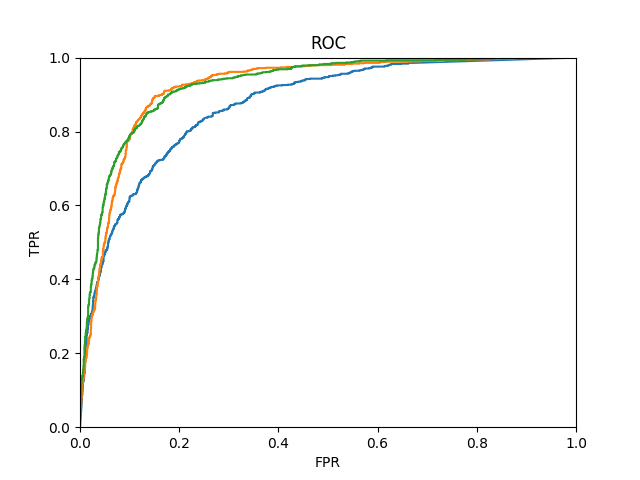
\includegraphics[width=.4\textwidth]{LR.png}
\caption{Logistics Regression}
\end{figure}

\subsection{Decision Tree}
\quad A decision tree is a diagram or chart that people use to determine a course of action or show a statistical probability. It forms the outline of the namesake woody plant, usually upright but sometimes lying on its side. Each branch of the decision tree represents a possible decision, outcome, or reaction. The farthest branches on the tree represent the end results.

As is shwon below, decision tree is much more powerful than any other model we used. ROC of decision tree is red.


\begin{figure}[H]
\centering
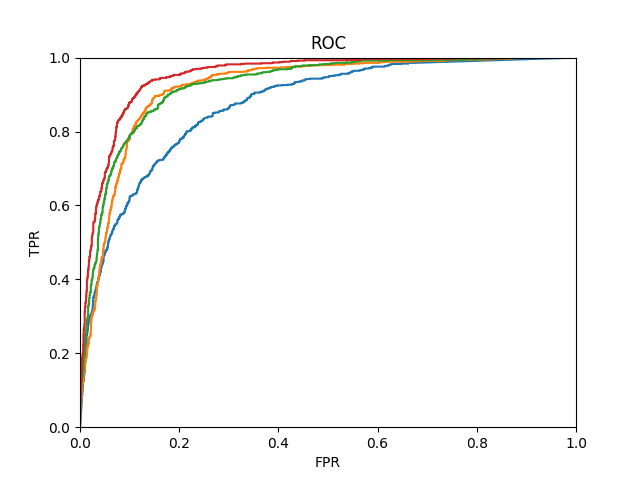
\includegraphics[width=.4\textwidth]{XGB.png}
\caption{Decision Tree}
\end{figure}


\subsection{Gradient Boosting}
\quad Gradient boosting machines are a family of powerful machine-learning techniques that have shown considerable success in a wide range of practical applications. They are highly customizable to the particular needs of the application, like being learned with respect to different loss functions.

 But nothing goes smoothly, what depressed us it that gradient boosting is not as good as decision tree(red). ROC of gradient boosting is purple.
\begin{figure}[H]
\centering
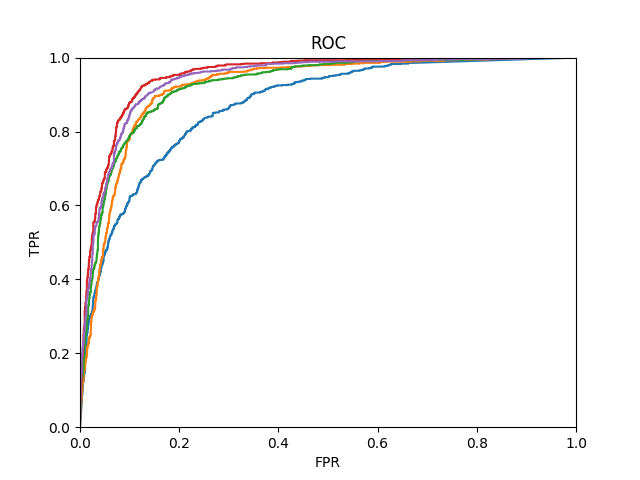
\includegraphics[width=.4\textwidth]{GB.png}
\caption{Gradient Boosting}
\end{figure}

\subsection{Random Forests}
\quad Random forests are a combination of tree predictors such that each tree depends on the values of a random vector sampled independently and with the same distribution for all trees in the forest. The generalization error for forests converges a.s. to a limit as the number of trees in the forest becomes large. The generalization error of a forest of tree classifiers depends on the strength of the individual trees in the forest and the correlation between them. 

The performance of random forests is the same as decision tree(red) almost surely. ROC of random forests is brown.
\begin{figure}[H]
\centering
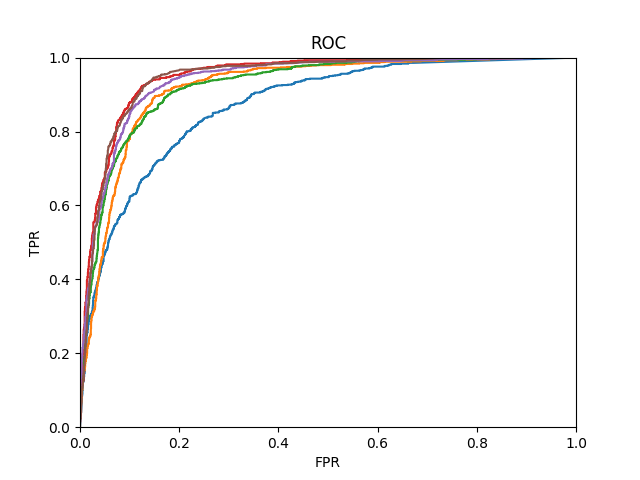
\includegraphics[width=.4\textwidth]{RF.png}
\caption{Random Forests}
\end{figure}

\subsection{Summary}
\quad After combining these non-sequential models with ensemble method, we can beat the moderate line. But it seems that we have got a bottleneck. After all, the method based on frequency have discarded some important information. So we turn to sequential model to get improved.



\section{Sequential Model}
\quad In this section, we mainly talk about Convolutional Neural Networks because it's one of the most widely used technique in deep learning.

\subsection{Overview}
\quad Convolutional Neural Networks (CNN) are biologically-inspired variants of MLPs. From Hubel and Wiesel’s early work on the cat’s visual cortex [Hubel68], we know the visual cortex contains a complex arrangement of cells. These cells are sensitive to small sub-regions of the visual field, called a receptive field. The sub-regions are tiled to cover the entire visual field. These cells act as local filters over the input space and are well-suited to exploit the strong spatially local correlation present in natural images.

\begin{figure}[H]
\centering
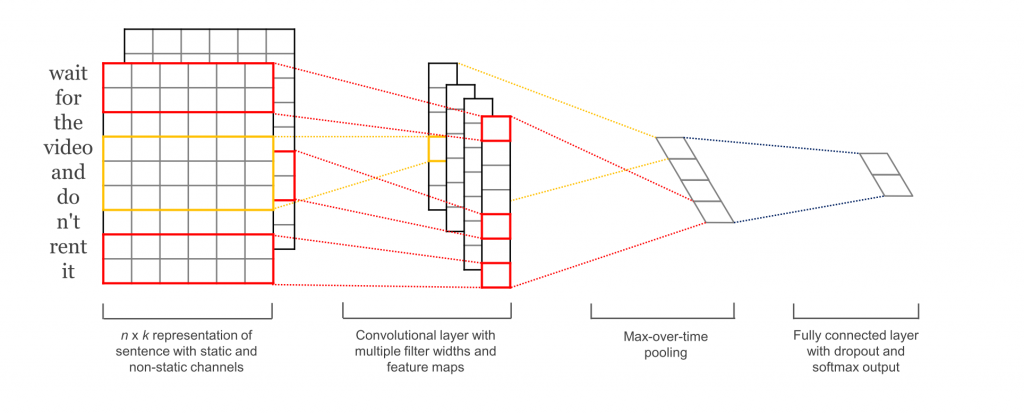
\includegraphics[width=.4\textwidth]{1.png}
\caption{A Sketch of CNN}
\end{figure}

Additionally, two basic cell types have been identified: Simple cells respond maximally to specific edge-like patterns within their receptive field. Complex cells have larger receptive fields and are locally invariant to the exact position of the pattern.

\subsection{Convolutional Layer}
\quad The brain view: If you’re a fan of the brain/neuron analogies, every entry in the 3D output volume can also be interpreted as an output of a neuron that looks at only a small region in the input and shares parameters with all neurons to the left and right spatially (since these numbers all result from applying the same filter). We now discuss the details of the neuron connectivities, their arrangement in space, and their parameter sharing scheme.

\begin{figure}[H]
\centering
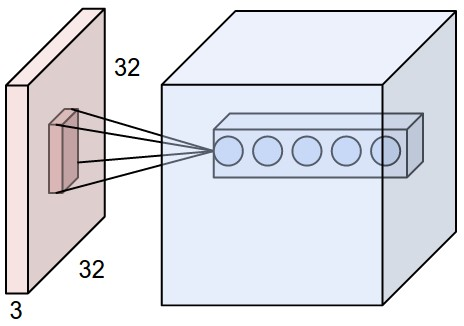
\includegraphics[width=.2\textwidth]{depthcol.jpeg}
\caption{An example }
\end{figure}

\subsection{Pooling Layer}

\quad A key aspect of Convolutional Neural Networks are pooling layers, typically applied after the convolutional layers. Pooling layers subsample their input. The most common way to do pooling it to apply a max operation to the result of each filter. 

You don’t necessarily need to pool over the complete matrix, you could also pool over a window. For example, the following shows max pooling for a 2x2 window (in NLP we typically are apply pooling over the complete output, yielding just a single number for each filter)


Why pooling? There are a couple of reasons. One property of pooling is that it provides a fixed size output matrix, which typically is required for classification. For example, if you have 1,000 filters and you apply max pooling to each, you will get a 1000-dimensional output, regardless of the size of your filters, or the size of your input. This allows you to use variable size sentences, and variable size filters, but always get the same output dimensions to feed into a classifier.

\begin{figure}[H]
\centering
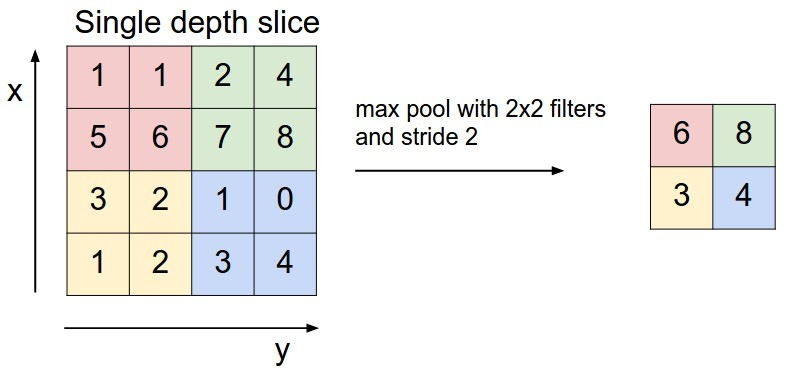
\includegraphics[width=.4\textwidth]{maxpool.jpeg}
\caption{Max Pooling}
\end{figure}

Pooling also reduces the output dimensionality but (hopefully) keeps the most salient information. You can think of each filter as detecting a specific feature, such as detecting if the sentence contains a negation like “not amazing” for example. If this phrase occurs somewhere in the sentence, the result of applying the filter to that region will yield a large value, but a small value in other regions. 

\begin{figure}[H]
\centering
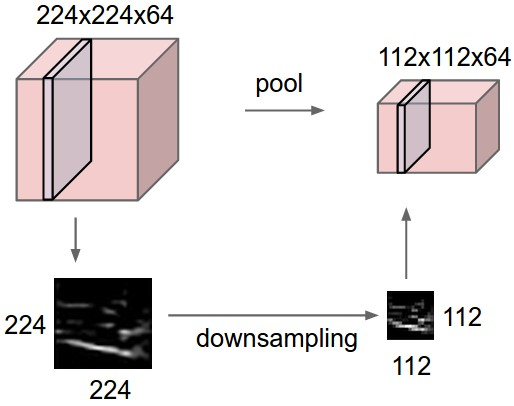
\includegraphics[width=.2\textwidth]{pool.jpeg}
\caption{Pooling layer downsamples}
\end{figure}

By performing the max operation you  are keeping information about whether or not the feature appeared in the sentence, but you are losing information about where exactly it appeared. But isn’t this information about locality really useful? Yes, it  is and it’s a bit similar to what a bag of n-grams model is doing. You are losing global information about locality (where in a sentence something happens), but you are keeping local information captured by your filters, like “not amazing” being very different from “amazing not”.

\subsection{Normalization Layer}

\quad Many types of normalization layers have been proposed for use in ConvNet architectures, sometimes with the intentions of implementing inhibition schemes observed in the biological brain. However, these layers have since fallen out of favor because in practice their contribution has been shown to be minimal, if any. For various types of normalizations, see the discussion in Alex Krizhevsky’s cuda-convnet library API.

\subsection{Fully-connected layer}

\quad Neurons in a fully connected layer have full connections to all activations in the previous layer, as seen in regular Neural Networks. Their activations can hence be computed with a matrix multiplication followed by a bias offset. See the Neural Network section of the notes for more information.

\subsection{Dropout Layer}
\quad Dropout is the perhaps most popular method to regularize convolutional neural networks. The idea behind dropout is simple. A dropout layer stochastically “disables” a fraction of its neurons. This prevent neurons from co-adapting and forces them to learn individually useful features. The fraction of neurons we keep enabled is defined by the dropout keep prob input to our network. We set this to something like 0.5 during training, and to 1 (disable dropout) during evaluation.

\subsection{Sparse Connectivity}
\quad CNNs exploit spatially-local correlation by enforcing a local connectivity pattern between neurons of adjacent layers. In other words, the inputs of hidden units in layer m are from a subset of units in layer m-1, units that have spatially contiguous receptive fields. We can illustrate this graphically as follows:


\begin{figure}[H]
\centering
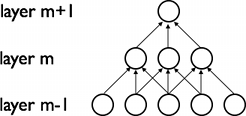
\includegraphics[width=.2\textwidth]{sparse_1D_nn.png}
\caption{Sparse Connectivity in Conv 1D NN}
\end{figure}

Imagine that layer m-1 is the input retina. In the above figure, units in layer m have receptive fields of width 3 in the input retina and are thus only connected to 3 adjacent neurons in the retina layer. Units in layer m+1 have a similar connectivity with the layer below. We say that their receptive field with respect to the layer below is also 3, but their receptive field with respect to the input is larger (5). Each unit is unresponsive to variations outside of its receptive field with respect to the retina. The architecture thus ensures that the learnt “filters” produce the strongest response to a spatially local input pattern.

However, as shown above, stacking many such layers leads to (non-linear) “filters” that become increasingly “global” (i.e. responsive to a larger region of pixel space). For example, the unit in hidden layer m+1 can encode a non-linear feature of width 5 (in terms of pixel space).

\subsection{Shared Weights}

\quad In addition, in CNNs, each filter hi is replicated across the entire visual field. These replicated units share the same parameterization (weight vector and bias) and form a feature map.



In the above figure, we show 3 hidden units belonging to the same feature map. Weights of the same color are shared—constrained to be identical. Gradient descent can still be used to learn such shared parameters, with only a small change to the original algorithm. The gradient of a shared weight is simply the sum of the gradients of the parameters being shared.

\begin{figure}[H]
\centering
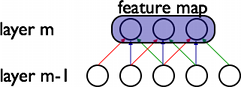
\includegraphics[width=.2\textwidth]{conv_1D_nn.png}
\caption{Shared Weights in Conv 1D NN}
\end{figure}

Replicating units in this way allows for features to be detected regardless of their position in the visual field. Additionally, weight sharing increases learning efficiency by greatly reducing the number of free parameters being learnt. The constraints on the model enable CNNs to achieve better generalization on vision problems.



\subsection{Character-Level CNNs}

\quad Character-Level CNN learns character-level embeddings, joins them with pre-trained word embeddings, and uses a CNN for Part of Speech tagging.  It explores the use of CNNs to learn directly from characters, without the need for any pre-trained embeddings. Notably, the authors use a relatively deep network with a total of 9 layers, and apply it to Sentiment Analysis and Text Categorization tasks. 

Results show that learning directly from character-level input works very well on large datasets (millions of examples), but underperforms simpler models on smaller datasets (hundreds of thousands of examples).It explores to application of character-level convolutions to Language Modeling, using the output of the character-level CNN as the input to an LSTM at each time step. The same model is applied to various languages.


\subsection{Model Design}
\quad The first layers embeds words into low-dimensional vectors. The next layer performs convolutions over the embedded word vectors using multiple filter sizes. For example, sliding over 3, 4 or 5 words at a time. Next, we max-pool the result of the convolutional layer into a long feature vector, add dropout regularization, and classify the result using a softmax layer.

\begin{figure}[H]
\centering
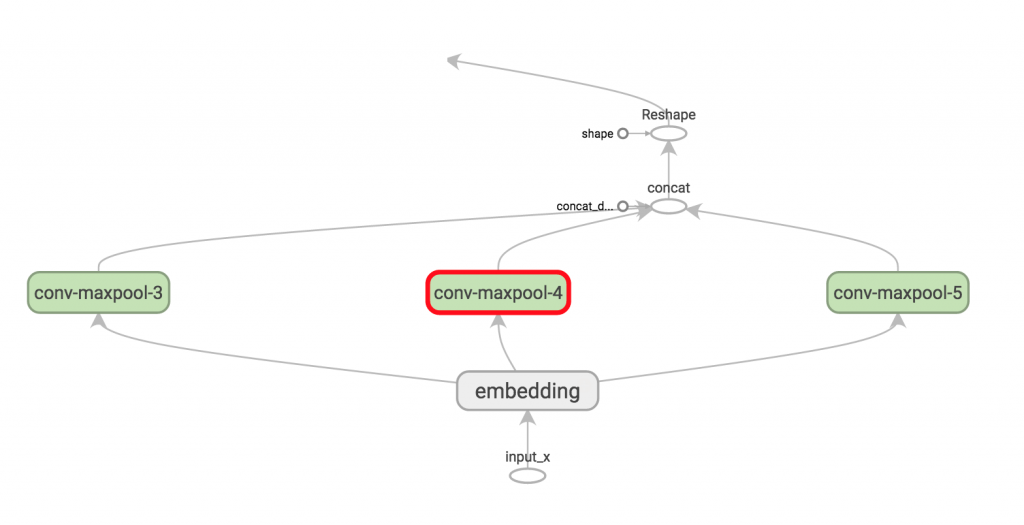
\includegraphics[width=.4\textwidth]{2.png}
\caption{Layout of the Neural Network}
\end{figure}


\begin{figure}[H]
\centering
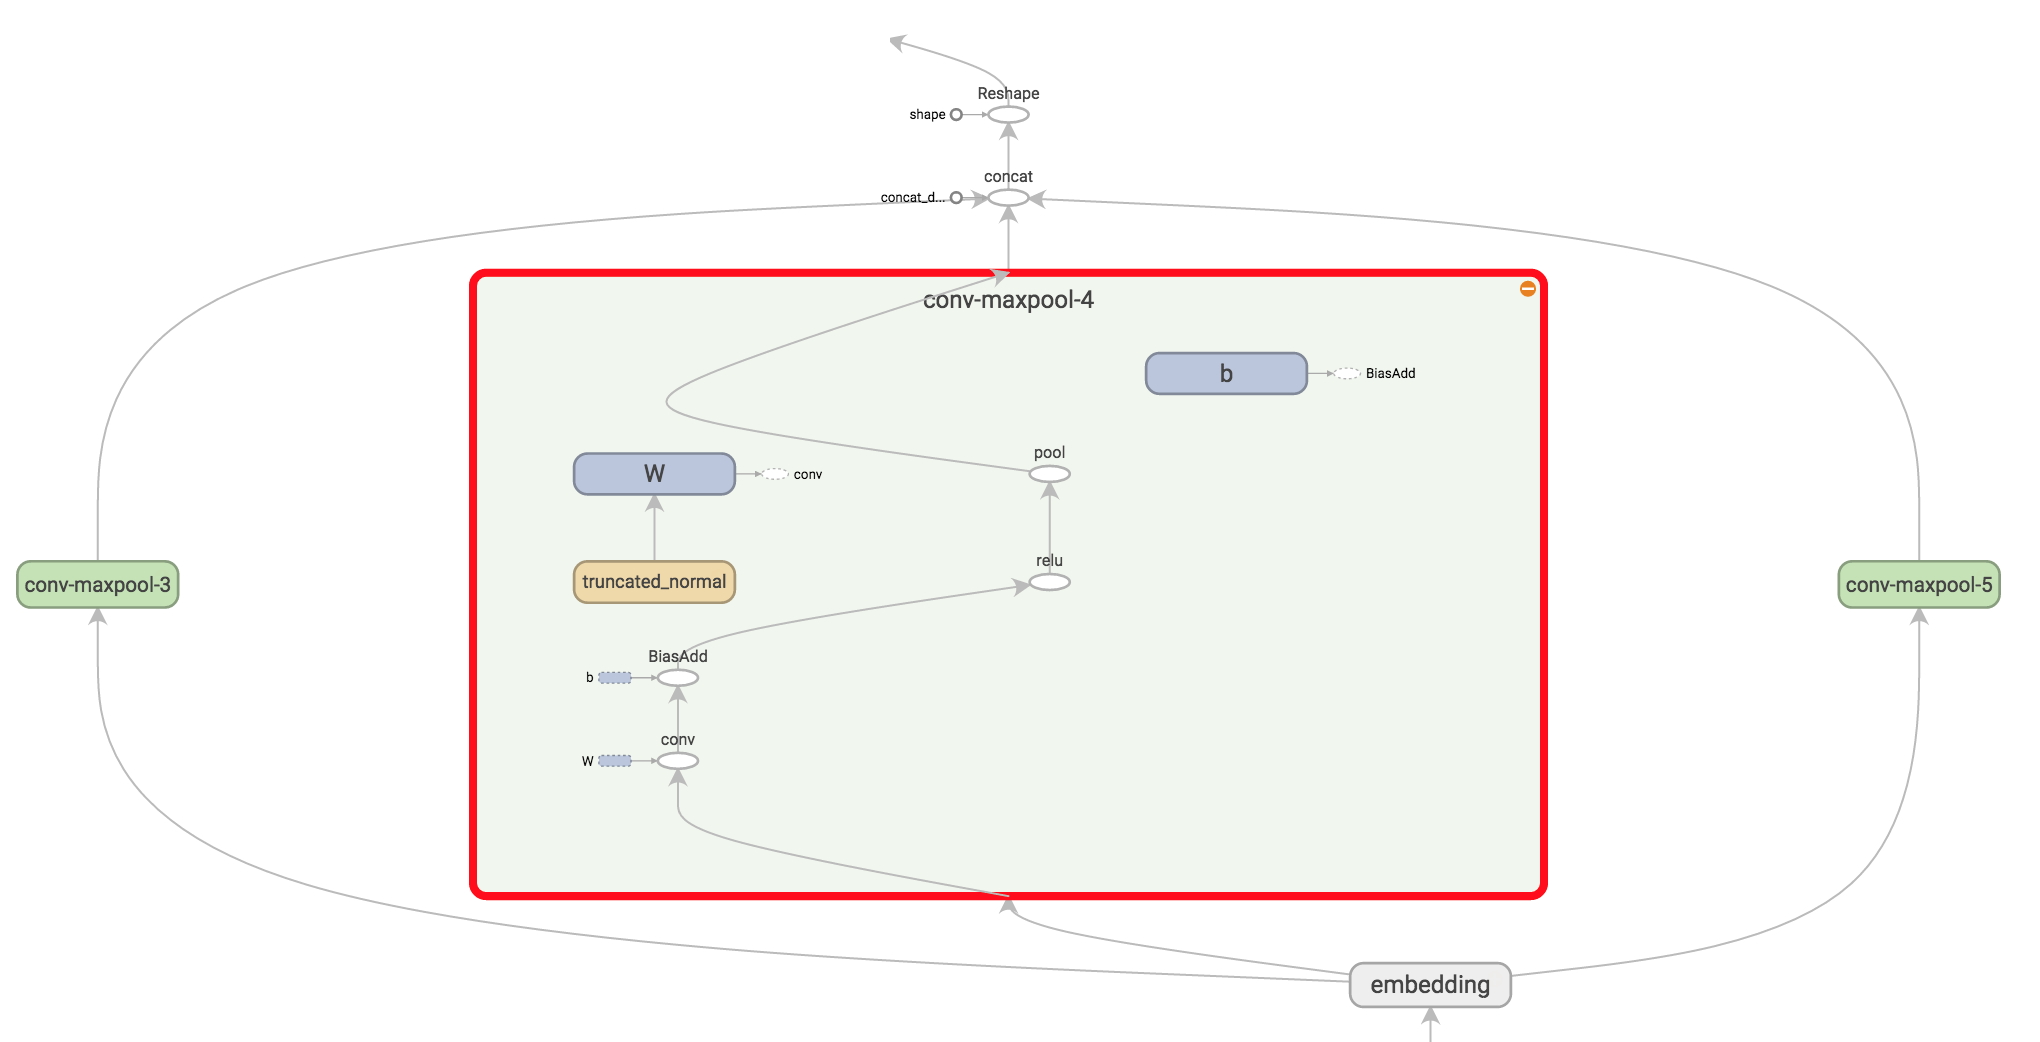
\includegraphics[width=.4\textwidth]{AM.png}
\caption{Detail of Conv-Maxpool}
\end{figure}

\subsection{Summary}
\quad With convolutional neural networks, our model shows great performance. What's more, it's very adaptive due to the fact that it runs even better on private cases.

\begin{figure}[H]
\centering
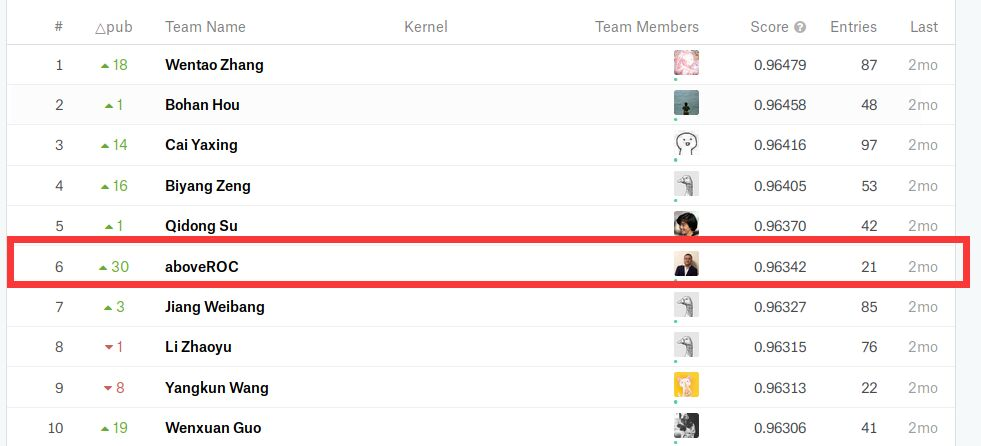
\includegraphics[width=.4\textwidth]{3.jpg}
\caption{Final Results}
\end{figure}

\section{Reference}

\quad    [1] Kim, Y. (2014). Convolutional Neural Networks for Sentence Classification. Proceedings of the 2014 Conference on Empirical Methods in Natural Language Processing (EMNLP 2014), 1746–1751.

    [2] Kalchbrenner, N., Grefenstette, E.,  Blunsom, P. (2014). A Convolutional Neural Network for Modelling Sentences. Acl, 655–665.

    [3] Santos, C. N. dos,  Gatti, M. (2014). Deep Convolutional Neural Networks for Sentiment Analysis of Short Texts. In COLING-2014 (pp. 69–78).

    [4] Johnson, R.,  Zhang, T. (2015). Effective Use of Word Order for Text Categorization with Convolutional Neural Networks. To Appear: NAACL-2015, (2011).

    [5] Johnson, R.,  Zhang, T. (2015). Semi-supervised Convolutional Neural Networks for Text Categorization via Region Embedding.

    [6] Wang, P., Xu, J., Xu, B., Liu, C., Zhang, H., Wang, F.,  Hao, H. (2015). Semantic Clustering and Convolutional Neural Network for Short Text Categorization. Proceedings ACL 2015, 352–357.

    [7] Zhang, Y.,  Wallace, B. (2015). A Sensitivity Analysis of (and Practitioners’ Guide to) Convolutional Neural Networks for Sentence Classification,

    [8] Nguyen, T. H.,  Grishman, R. (2015). Relation Extraction: Perspective from Convolutional Neural Networks. Workshop on Vector Modeling for NLP, 39–48.

    [9] Sun, Y., Lin, L., Tang, D., Yang, N., Ji, Z.,  Wang, X. (2015). Modeling Mention , Context and Entity with Neural Networks for Entity Disambiguation, (Ijcai), 1333–1339.

    [10] Zeng, D., Liu, K., Lai, S., Zhou, G.,  Zhao, J. (2014). Relation Classification via Convolutional Deep Neural Network. Coling, (2011), 2335–2344. 

    [11] Gao, J., Pantel, P., Gamon, M., He, X.,  Deng, L. (2014). Modeling Interestingness with Deep Neural Networks.

    [12] Shen, Y., He, X., Gao, J., Deng, L.,  Mesnil, G. (2014). A Latent Semantic Model with Convolutional-Pooling Structure for Information Retrieval. Proceedings of the 23rd ACM International Conference on Conference on Information and Knowledge Management – CIKM ’14, 101–110.

    [13] Weston, J.,  Adams, K. (2014).  T AG S PACE : Semantic Embeddings from Hashtags, 1822–1827.

    [14] Santos, C.,  Zadrozny, B. (2014). Learning Character-level Representations for Part-of-Speech Tagging. Proceedings of the 31st International Conference on Machine Learning, ICML-14(2011), 1818–1826. 

    [15] Zhang, X., Zhao, J.,  LeCun, Y. (2015). Character-level Convolutional Networks for Text Classification, 1–9.

    [16] Zhang, X.,  LeCun, Y. (2015). Text Understanding from Scratch. arXiv E-Prints, 3, 011102.

    [17] Kim, Y., Jernite, Y., Sontag, D.,  Rush, A. M. (2015). Character-Aware Neural Language Models.



\end{document}